There are jobs that are trivial for all people, even for kids, but they are extremely difficult even for the most powerful and sophisticated software and software. This type of task has as its characteristics the need for creativity and level of abstraction which, in the present moment, is slightly in the minds of human beings. Some examples classify this type of task with image recognition, especially when there is occlusion or involves subjective analysis, content authorship, analysis of emotions and so many other activities that inherently require human intelligence to be performed. Luis von Ahn introduced in his dissertation  \cite{VonAhn:2005:HC:1168246}  a paradigm named Human Computation (HC) that allows to approach the problems from this point of view, identifying in it what tasks can be automated and which are those that require human treatment. Additionaly HC can improve performance by division of labor because it helps to define tasks that can be executed in parallel \cite{Rohwer:2010:NHC:1837885.1837897}.

One of the benefits of modeling a system according to the HC paradigm is to focus the effort of human collaborators only on tasks that really require their attention, this is done by identifying the tasks that inherently require human intelligence. Each of these tasks is a HIT (Human Intelligence Task) and corresponds to something that humans can easily solve while a machine presents extreme difficulty in trying to solve \cite{doi:10.2200/S00371ED1V01Y201107AIM013}. Three renowned projects that were conceived based on Human Computing are reCAPTCHA \cite{Simmons:2010:PLV:1869086.1869102}, ESP Game \cite{Robertson:2009:REG:1520340.1520597}, and Duolingo \cite{vonAhn:2011:THC}.

\begin{figure}[!htb]
\centering
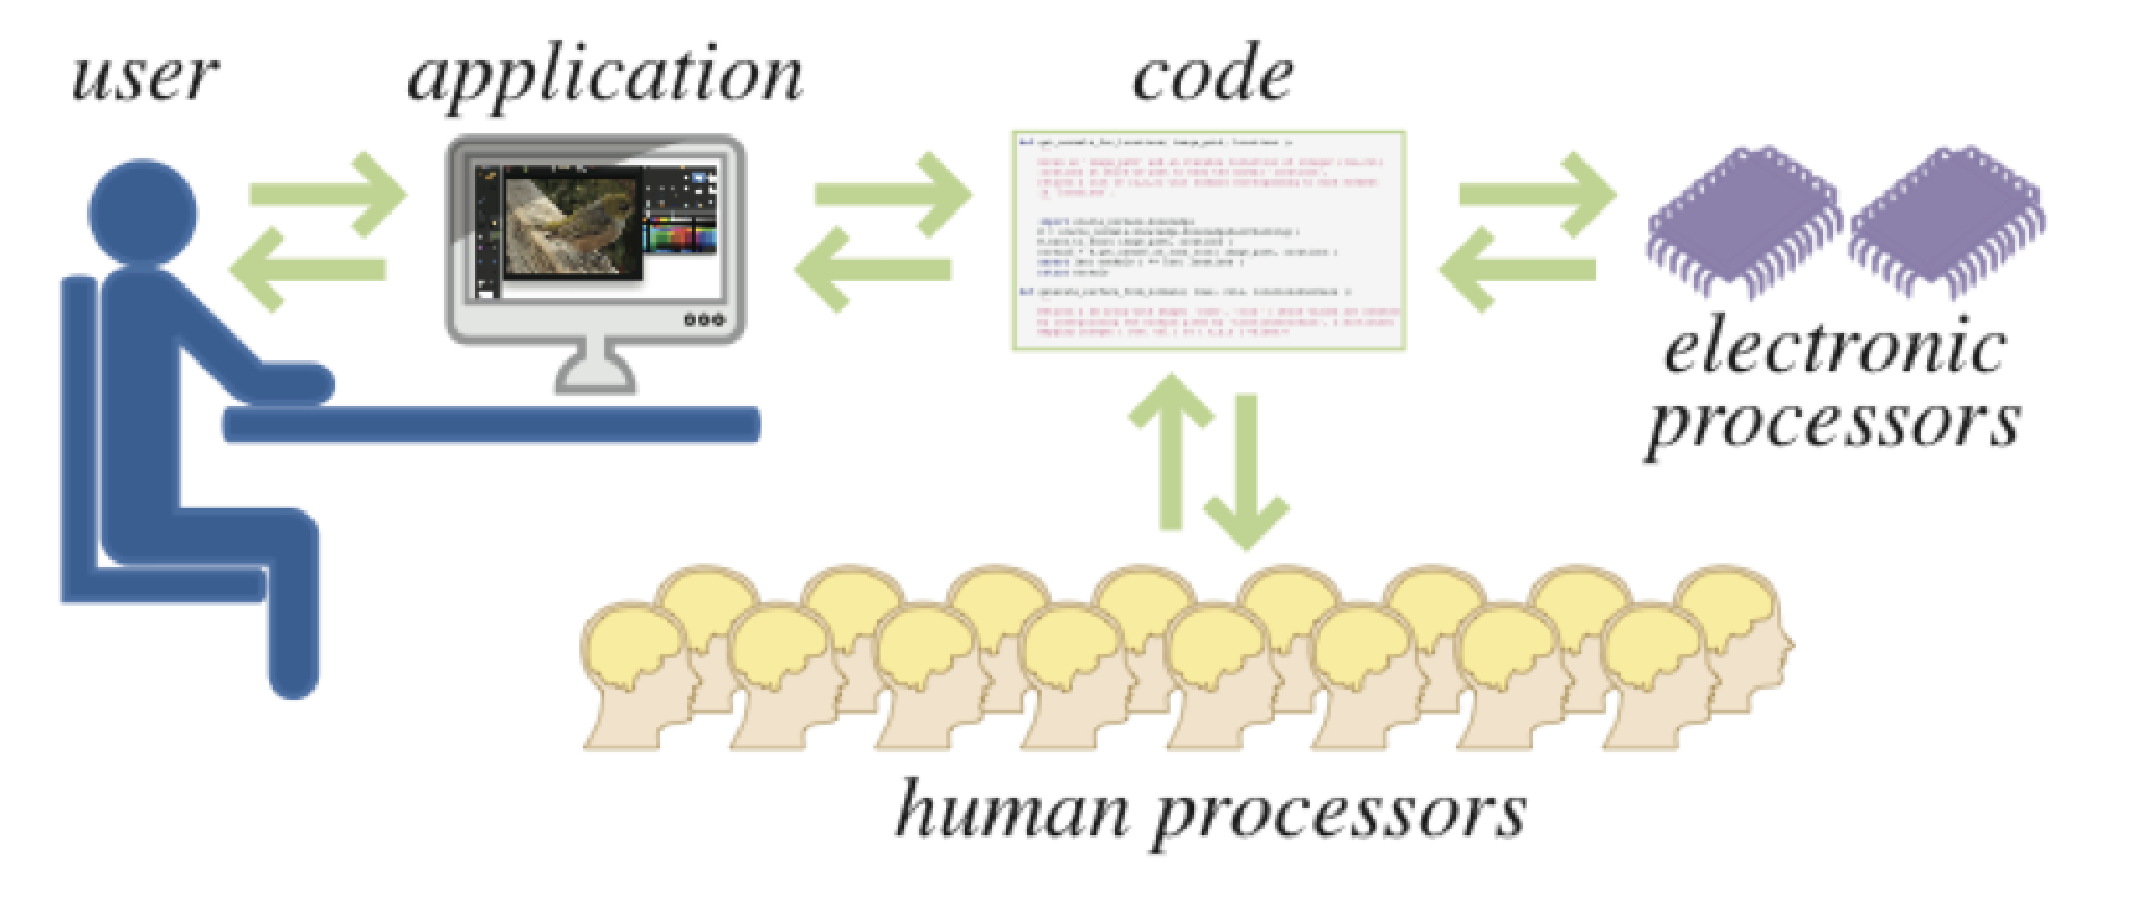
\includegraphics[scale=0.2]{figure/hc}
\caption{Human Computation - REFAZER FIGURA}
\label{Human Computation}
\end{figure}

The Esp Game was a system, modeled as an online game, which had as its internal goal to collect labels on images that were presented randomly to users. In this way it was possible to create an annotated base of images with several annotations that any human could write, which a computer could hardly obtain because of occlusion, discharacterization form and necessity of interpretation of context or subjective inference \cite{Robertson:2009:REG:1520340.1520597,vonAhn:2008:DGP:1378704.1378719}. Google subsequently purchased a system license and used it as the basis for its own version, Google Image Labeler\cite{1_saini_2017}. Google Image Labeler has been discontinued in 2013 and was brought back in 2016 \cite{3_backchitu_2017}.  Additionally, is an initiative of the Institute of Art History at the University of Munich which currently uses a system based on The ESP Game to create a digital annotated image base that refers to its art collection \cite{2_muumlnchen_2017}.


CAPTCHA (Completely Automated Public Turing test to tell Computers and Humans Apart) tests are a very efficient way of determining if a particular requirement is being made by a human user or by some type of robot \cite{Simmons:2010:PLV:1869086.1869102}. Based on this premise, Luis von Ahn had an interesting idea of incorporating into them small tasks that require human intelligence. This idea originated reCAPTCHA, which uses the strategy of reshaping CAPTCHA tests so that human intelligence used by users can be used to support applications such as text recognition in situations where automatic systems present major difficulties  \cite{Ahn08recaptcha:human-based}.

Duolingo has as one of its objectives to translate texts using human intelligence instead of automatic methods. In this environment users translate texts while they learn, and the texts presented are selected from the dataset that one wants to translate \cite{vonAhn:2011:THC}. Translation is another application that despite count on automatic techniques presents situations where it is necessary that human intelligence be used to generate a result within the relevant quality \cite{bywood2017embracing}. Automatic translation faces serious difficulties related to context, slangs, language expressions, regionalisms among others, while humans can deal with relative ease with these questions \cite{guerra2000machine}.

In short, Human Computation is a paradigm that proposes to identify into the problems which tasks require human intelligence and which tasks can be automated. In general, it may be benefited with modeling based on the Human Computation paradigm the problems in which it is possible to identify tasks that are very difficult for machines but which can be easily completed by humans.


